\subsection{Unpacking the Joy of Ground Gain!}

\begin{tcolorbox}[colback=gray!10, colframe=black, title=E9A05] What does the term “ground gain” mean?
\begin{enumerate}[label=\Alph*.]
    \item The change in signal strength caused by grounding the antenna
    \item The gain of the antenna with respect to a dipole at ground level
    \item To force net gain to 0 dB by grounding part of the antenna
    \item \textbf{An increase in signal strength from ground reflections in the environment of the antenna}
\end{enumerate} \end{tcolorbox}

\subsubsection{Related Concepts}

Ground gain refers to the increase in signal strength achieved due to reflections from the ground under specific conditions. When an antenna is situated close to the ground, incoming signals can reflect off the ground, leading to a constructive interference effect that enhances the overall signal strength received by the antenna. This phenomenon is particularly relevant in radio wave propagation, where understanding how various surfaces affect signal transmission is crucial.

\subsubsection{Key Concepts Required}

To fully grasp the concept of ground gain, one should be familiar with:
\begin{itemize}
    \item Antenna theory—how antennas radiate and receive electromagnetic waves.
    \item Signal propagation—specifically, how signals travel through different mediums (air, ground).
    \item Reflection and interference patterns—how waves can constructively or destructively interfere with one another.
\end{itemize}

\subsubsection{Mathematical Considerations}

Ground gain can often be estimated by considering the environmental factors affecting signal propagation. If \( G \) is the ground gain, it can be expressed in dB as:

\[
G = 10 \log_{10}\left(\frac{P_{\text{reflected}}}{P_{\text{incident}}}\right)
\]

Where:
- \( P_{\text{reflected}} \) is the power of the signal received due to reflections,
- \( P_{\text{incident}} \) is the power of the direct signal.

This formula shows how the power gain, in decibels, is related to the ratio of the reflected power to the incident power from the antenna.

\subsubsection{Diagram}

To better understand ground gain, consider depicting a simple diagram using TikZ. The following code provides a basic illustration of an antenna receiving signals from both the direct path and reflected path:

\begin{center}
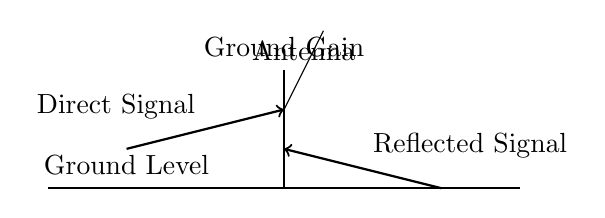
\begin{tikzpicture}
    % Draw the ground
    \draw[thick] (-3,0) -- (3,0);

    % Draw the antenna
    \draw[thick] (0,1.5) -- (0,0);
    \draw[-] (0,1) -- (0.5,2) node[midway, above] {Antenna};

    % Direct signal
    \draw[->, thick] (-2,0.5) -- (0,1) node[midway, above left] {Direct Signal};

    % Reflected signal
    \draw[->, thick] (2,0) -- (0,0.5) node[midway, above right] {Reflected Signal};

    % Labels
    \node at (-2, 0.3) {Ground Level};
    \node at (0, 1.8) {Ground Gain};
\end{tikzpicture}
\end{center}

In summary, understanding ground gain involves recognizing how reflections from the ground can enhance the performance of antennas, underscoring the importance of position and environmental factors in communication systems.
